\documentclass[12pt,a4paper]{article}
\usepackage{amsmath}
\usepackage{float}
\usepackage{amsfonts}
\usepackage{url}
\usepackage{tcolorbox}
\usepackage{array}
\usepackage{amssymb}
\usepackage{graphicx}
\usepackage[left=2cm,right=2cm,top=2cm,bottom=2cm]{geometry}

\title{\textbf{ASSIGNMENT-4 \\ ID2090}} 
\author{Rhythem Sood}
\date{17th June, 2023}

\begin{document}

\maketitle

\begin{table}[H]
\centering
\setlength{\extrarowheight}{5pt}
\begin{tabular}{|p{6cm}|p{6cm}|}
\hline
\textbf{Name}          & \textbf{Rhythem Sood} \\ \hline
\textbf{Roll No.}      & \textbf{MM22B051}     \\ \hline
\textbf{Github Username} & \textbf{mm22b051}     \\ \hline
\end{tabular}
\end{table}

\begin{center}
   \section*{Thermal Expansion} 
\end{center}
Thermal Expansion refers to the property of a material that involves a change in length, area, volume, and density with temperature change.
\cite{wiki} \\ 
The main reason for thermal expansion is the increase in kinetic energy of the constituent particles with the increase in temperature. As their kinetic energy increases, the particles tend to move with greater velocity and hence require more space, leading to an increase in shape or size. 
\begin{itemize}
    \item 
    The linear thermal expansion equation is given by:
    \vspace{6pt}
    \begin{center}
        \begin{tcolorbox}[width=10cm,colback=white]
            \begin{equation}
            \centering
            \frac{dL}{L} = \alpha \cdot {dT}
            \end{equation}
        \end{tcolorbox} 
    \end{center}
    \item 
    The surface thermal expansion equation is given by:
    \vspace{6pt}
    \begin{center}
        \begin{tcolorbox}[width=10cm,colback=white]
            \begin{equation}
            \centering
            \frac{dA}{A} = \beta \cdot {dT}
            \end{equation}
        \end{tcolorbox} 
    \end{center}
    \item 
    The volume thermal expansion equation is given by:
    \vspace{6pt}
    \begin{center}
        \begin{tcolorbox}[width=10cm,colback=white]
            \begin{equation}
            \centering
            \frac{dV}{V} = \gamma \cdot {dT}
            \end{equation}
        \end{tcolorbox} 
    \end{center}
\end{itemize}
where;\\ $\alpha, \beta, \gamma$ are the linear, surface, volume thermal expansion coefficients respectively, \\
$dL, dA, dV$ is the change in length, area and volume respectively \\
$L, A, V$ is the original length, area and volume respectively \\
$dT$ is the temperature change. 

\section{Graph for Linear Thermal Expansion Coefficient }
\cite{Allvar}
\begin{figure}[H]
    \begin{center}
     \framebox{
        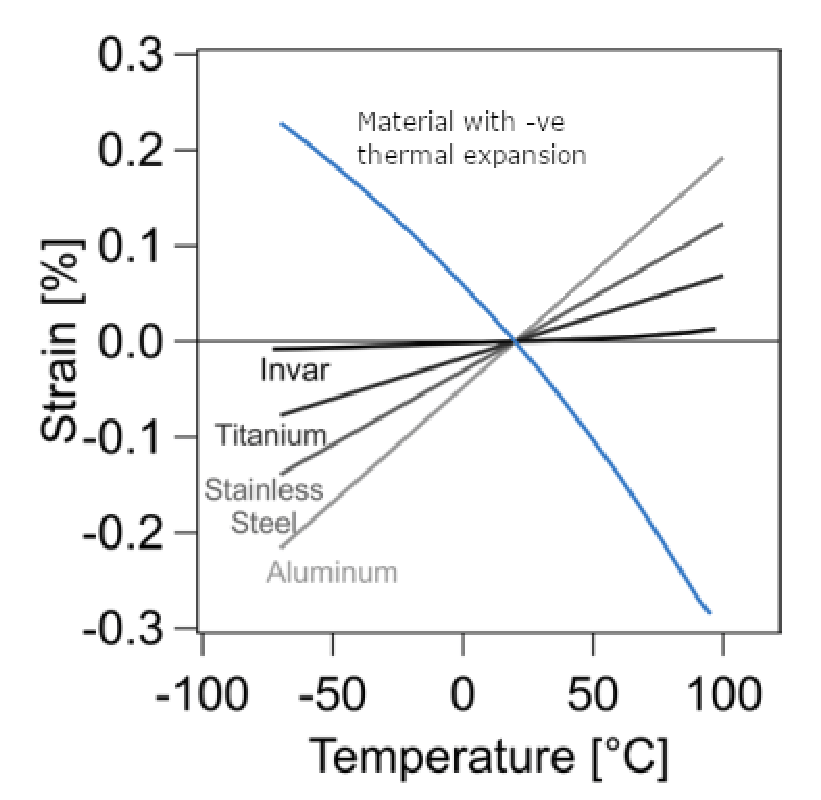
\includegraphics
        {1.eps}
     }
    \end{center}
    \caption{Plot of strain vs temperature}
\end{figure}

\section{Reason for choosing this equation}
 
This equation is fundamental in understanding how materials respond to changes in temperature, as it provides insights into the shape and size alterations with temperature. It is an essential property of materials and holds significant importance in analyzing various materials. Although we may have encountered this equation in our earlier academic years, revisiting it in our MM1001 course(i.e. MM department introductory course) shows how relevant it is and tells about its practical applications in our department. Thus, I recognized it as a significant equation and chose it for my assignment.

\bibliography{ref}
\bibliographystyle{alpha}
\end{document}

